%%%%%%%%%%%%%%%%%%%%%%%%%%%%%%%%%%%%%%%%%
% University/School Laboratory Report
% LaTeX Template
% Version 3.1 (25/3/14)
%
% This template has been downloaded from:
% http://www.LaTeXTemplates.com
%
% Original author:
% Linux and Unix Users Group at Virginia Tech Wiki 
% (https://vtluug.org/wiki/Example_LaTeX_chem_lab_report)
%
% License:
% CC BY-NC-SA 3.0 (http://creativecommons.org/licenses/by-nc-sa/3.0/)
%
%%%%%%%%%%%%%%%%%%%%%%%%%%%%%%%%%%%%%%%%%

%----------------------------------------------------------------------------------------
%	PACKAGES AND DOCUMENT CONFIGURATIONS
%----------------------------------------------------------------------------------------

\documentclass{article}

%\usepackage[version=3]{mhchem} % Package for chemical equation typesetting
%\usepackage{siunitx} % Provides the \SI{}{} and \si{} command for typesetting SI units
\usepackage{graphicx} % Required for the inclusion of images
%\usepackage{natbib} % Required to change bibliography style to APA
%\usepackage{amsmath} % Required for some math elements 
\usepackage{listings}
\lstset{
  breaklines=true,
  basicstyle=\scriptsize,
  columns=fullflexible
}

\usepackage{tikz}

\setlength\parindent{0pt} % Removes all indentation from paragraphs

%\renewcommand{\labelenumi}{\alph{enumi}.} % Make numbering in the enumerate environment by letter rather than number (e.g. section 6)

%\usepackage{times} % Uncomment to use the Times New Roman font

%----------------------------------------------------------------------------------------
%	DOCUMENT INFORMATION
%----------------------------------------------------------------------------------------

\title{Report: Homework 8 - MapReduce (Hadoop) with Povray}% Title

\author{Jan \textsc{Schlenker} \& Sebastian \textsc{Sams}} % Author name

\date{\today} % Date for the report

\begin{document}

\maketitle % Insert the title, author and date

\begin{center}
\begin{tabular}{l l}
Instructor: & Dipl.-Ing. Dr. Simon Ostermann \\
Programming language: & Java \\
Library used: & Hadoop 2.4.0 \& Java AWS SDK 1.10.0 \\
Total points: & 50 \\
\end{tabular}
\end{center}

% If you wish to include an abstract, uncomment the lines below
% \begin{abstract}
% Abstract text
% \end{abstract}

%----------------------------------------------------------------------------------------
%	SECTION 1
%----------------------------------------------------------------------------------------

\section{Prerequisites}

\begin{itemize}
\item Java 1.7
\item Maven 3.0.5
\end{itemize}

\section{How to run the programme}

First of all extract the archive file homework\_8.tar.gz:

\begin{lstlisting}[language=bash, deletekeywords={cd}]
  $ tar -xzf homework_8.tar.gz
  $ cd homework_8
\end{lstlisting}

Afterwards move/copy the executable files povray and gm to map-reduce-povray/ src/resources/:

\begin{lstlisting}[language=bash]
  $ cp <gm-file-path> <povray-file-path> map-reduce-povray/src/resources/
\end{lstlisting}

The programme allows to render Povray files on a Hadoop cluster.
It is splitted into two subprogrammes:

\begin{enumerate}
\item map-reduce-povray: contains the the implementation of the Mapper and the Reducer
\item map-reduce-povray-ui: contains a gui implementation to start a MapReduce job in an AWS Elastic MapReduce (EMR) cluster
\end{enumerate}

First of all build all projects:

\begin{lstlisting}[language=bash, deletekeywords={cd}]
  $ mvn clean install
\end{lstlisting}

The map-reduce-povray programme can be executed on a local Hadoop cluster via:

\begin{lstlisting}[language=bash, deletekeywords={cd}]
  $ $HADOOP_HOME/bin/hadoop jar map-reduce-povray/target/map-reduce-povray-1.0.jar mapReducePovray.Povray <input-dir> <output-dir> <uri-of-pov-file>
\end{lstlisting}

The programme can also be executed on Amazon EMR. A small user interface for using it via EMR is available in the project map-reduce-povray-ui. Required preparations before running the user interface (applies to both the command line and GUI version):

\begin{itemize}
\item Create an EMR cluster, note the cluster ID
\item Create an S3 bucket and upload the jar-file containing the map-reduce implementation
\item Create access credentials which have permissions to create and monitor steps on the cluster and can list and edit files on the S3 bucket. Store them in a properties file called "AwsCredentials.properties" as entries named \emph{accessKey} and \emph{secretKey}.
\end{itemize}

The map-reduce-povray-ui GUI programme can be executed via:

\begin{lstlisting}[language=bash, deletekeywords={cd}]
  $ cd map-reduce-povray-ui
  $ mvn exec:java
\end{lstlisting}

\section{Programme explanation}

Figure~\ref{fig:map-reduce-povray-workflow} shows the MapReduce (Hadoop) workflow for Povray.

\begin{figure}[htbp]
\begin{center}
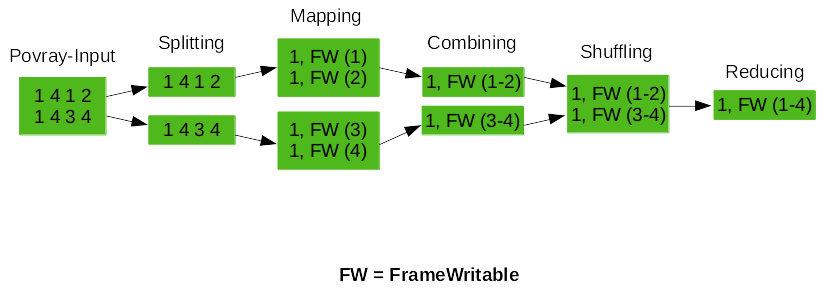
\includegraphics[width=\textwidth]{map-reduce-povray-workflow.png}
\caption{MapReduce (Hadoop) workflow for Povray}
\label{fig:map-reduce-povray-workflow}
\end{center}
\end{figure}

\subsection{Mapper}

The mapper processes take text files as input, whose first line must have the following structure:

\begin{lstlisting}[language=bash, deletekeywords={cd}]
  <start-frame> <end-frame> <subset-start-frame> <subset-end-frame>
\end{lstlisting}

Because the Povray file is part of the created jar, the mappers can simply create the subset-frames, pack them as FrameWritables (which is a custom implementation of the Mapper/Reducer output interface Writable) and output them one by one in the following format:

\begin{lstlisting}[language=bash, deletekeywords={cd}]
  1, FrameWritable(<frame-number>, "png", <bytes-of-frame>)
\end{lstlisting}

The key is always one, because one reducer is responsible for values with the same key and all pictures should be merged to one file.
The needed pov-file for the mapper processes is attached as a cache file by the main programme.

\subsection{Reducer (\& Combiner)}
In Hadoop the output of one mapper will first go into one combiner. The combiner works often as a pre-reducer and reduces the output of one mapper. In this programme the combiner and the reducer implementations are the same. The combiner first merges the rendered pictures of one mapper to a gif and outputs them to the shuffler. The shuffler on the other hand outputs all values with the same key to one reducer. Because there is only one key, the shuffler outputs always only one dataset, which contains all the pre-merged gifs. At last one reducer merges all pre-merged gifs to one.

\section{Performance}

To test the implementation, the well known \emph{scherk.pov} animation was rendered using Amazon EMR. A cluster using four \emph{m3.xlarge}\footnote{\emph{xlarge} instances are the smallest type of the current generation usable with Amazon EMR} instances as core instances and a single \emph{c3.xlarge} instance as a master was set up. In this setup 16 cores in total are available for rendering.

In the first tests \emph{c3.xlarge} instances were used for the rendering as they are slightly cheaper than the \emph{m3} counterparts and provide slightly better computational performance according to the Amazon specifications. However only two mapper tasks per node were run in parallel by the Hadoop scheduler, and the computational power of the nodes was therefore not utilized fully. Further investigation indicated that in the used version Hadoop uses multiple parameters such as available CPU cores and memory together with an estimation of required resources per task to decide on the actual number of parallel tasks. Therefore test were done again using \emph{m3.xlarge} instances which have the same number of CPU cores but twice the memory available. Hadoop scheduled six tasks per node in this configuration, which seemed appropriate. Hadoop introduces some overhead when managing the individual tasks; due to the maximum number of active tasks being slightly higher than the number of available CPU cores, the node should be utilized fully by the Povray processes most of the time.

The animation was rendered with a resolution of 1024x786 pixels. On the described cluster 300 frames could be rendered in approximately 8 minutes. The execution of the rendering job itself on the cluster was done in 7 minutes (timing data taken from EMR logs of the job execution). Data transfer and starting the job on the cluster add an additional minute which was not measured precisely as it primarily depends on the speed of the local internet connection and other parameters out of the scope of the implementation.

\end{document}
